\documentclass[root.tex]{subfiles}
\begin{document}


\section{Contrôle du bras Jaco dans le simulateur Gazebo par l'entremise de ROS}

Cette section traite d'un environnement de travail hautement versatile permettant la représentation de plusieur architectures de robots.
Pour les besoins du rapport, seulement un exemple avec le bras Jaco sera discuté.
De plus, la complexité de ROS et du simulateur Gazebo oblige de restreindre la présente section à la description sommaire des étapes nécessaires à la mise en marche de l'environnement et à l'utlisation de l'exemple fourni.
Les descriptions fournies ne cherchent pas à être fondamentalement exactes, mais plutôt à expliquer de manière intuitive et succincte le fonctionnement de l'infrastructure à des lecteurs non-initiés.
Il est important de noter que cet environnement est disponible seulement sur les plateformes Linux.

\subsection{Description de l'architecture générale de ROS}

ROS, \textit{robot operating system}, peut être décrit comme un ensemble de programmes (\textit{noeuds}) pouvant fonctionner de manière indépendante, entre lesquels des cannaux de communications standardisés sont établis.
Ces programmes communiquent entre eux en publiant l'information dans une liste des différents sujets (\textit{topics}) publiés par les noeuds présentement en fonctionnement.
Pour obtenir l'information publiée, un autre noeud peut s'abonner au sujet et ainsi lire l'information.

\subsection{Description du simulateur Gazebo}

Gazebo est un simulateur 3D pouvant fonctionner sans nécessiter l'instalation de ROS.
Cependant, il existe une version intégrée de Gazebo dans ROS Kinetic, la version de ROS utilisée pour Ubuntu 16.04.
Gazebo peut être vu comme un noeud ROS qui publie des informations par rapport aux différents composants de la simulation.
En utilisant le standard de fichier URDF, c'est dans ce programme que le robot est défini et que les contrôleurs des articulations sont créés.
Suivant la création du robot, Gazebo publie ainsi les informations de l'état du robot et s'abonne à des topics permettant la reception de commandes de moteurs.
La Figure \ref{fig:gazebo_jaco} représente l'interface du simulateur Gazebo lorsque le robot Jaco est configuré.

\begin{figure}
 \begin{center}
  \begin{tabular}{c}
    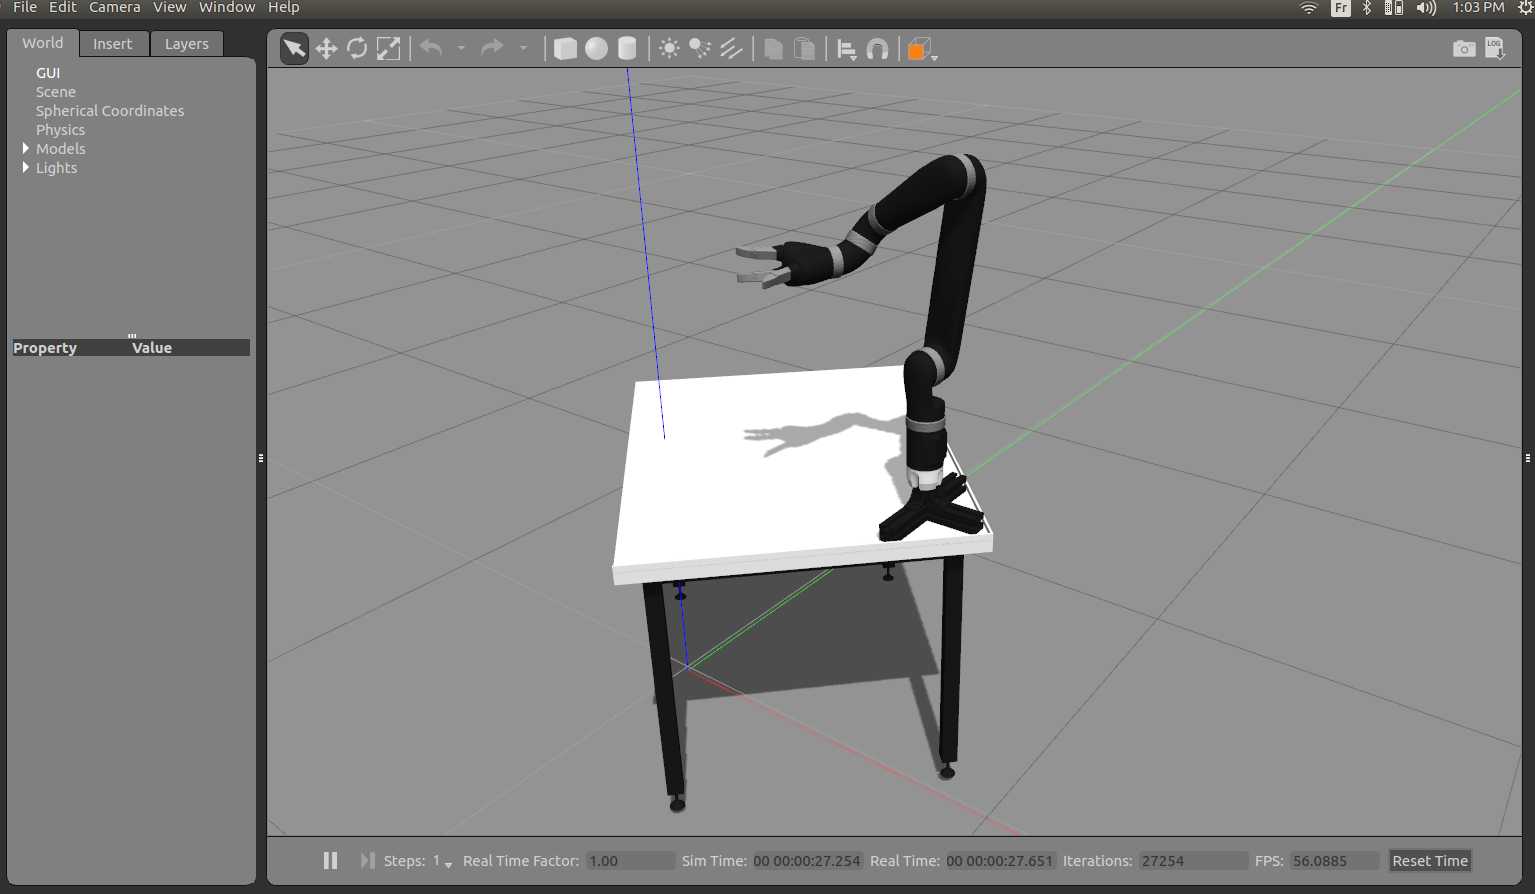
\includegraphics[trim=0cm 0cm 0cm 0cm, scale=0.25]{gazebo_jaco.png}
  \end{tabular}
 \end{center}
\caption{Interface du simulateur Gazebo avec le robot Jaco configuré}
 \label{fig:gazebo_jaco}
\end{figure}

La configuration du robot Jaco à été adaptée d'une suite de programmes (package) open-souce publiée par \cite{jaco_github}.

\subsection{Installation de ROS et de Gazebo}

Comme mentionné plus haut ROS est disponible seulement sur les systèmes d'exploitation Linux.
La séquence d'instructions suivante assume que le système d'exploitation Ubuntu 16.04 est fraichement installé.

\begin{itemize}
\item Aller sur le \href{http://wiki.ros.org/kinetic/Installation/Ubuntu}{site web suivant}.
\item Dans un invité de commande (terminal), entrer, dans l'ordre, les commandes aux étapes 1.2 et 1.3 du tutoriel.
\item Dans un terminal, entrer la commande: \textit{sudo apt-get install ros-kinetic-desktop-full}. Ceci installe ROS et Gazebo.
\item Dans un terminal, entrer, dans l'ordre, les commandes à l'étape 1.5 du tutoriel.
\item Dans un terminal, entrer la commande: echo "source /opt/ros/kinetic/setup.bash" $>>$ $\sim$/.bashrc
\item Entrer ensuite la commande: \textit{source $\sim$/.bashrc}
\item Dans un terminal, entrer la commande: \textit{sudo apt-get install ros-kinetic-catkin}. Ce programme permet la construction d'un environnement de travail avec ROS.
\item Aller sur le \href{http://wiki.ros.org/catkin/Tutorials/create_a_workspace}{site web suivant}.
\item Entrer les commandes mentionnée dans le tutoriel sur cette page.
\item Dans un terminal, entrer la commande: echo "source $\sim$/catkin\_ws/devel/setup.bash" $>>$ $\sim$/.bashrc
\item Entrer ensuite la commande: \textit{source $\sim$/.bashrc}
\end{itemize}

Après l'exécution de ces étapes, un environnement de travail pour ROS et Gazebo a été créé dans le fichier \textit{catkin\_ws} situé dans le répertoire \textit{home} de la plateforme Ubuntu.
Les fichiers sur lesquels le projet repose seront placés dans le sous-fichier \textit{src} de l'environnement de travail.

\subsection{Installation de la suite de programmes Jaco}

Après avoir installé ROS et Gazebo, il est maintenant possible de venir grèfer les modules permettant le contrôle d'un bras jaco en simulation.
Pour se faire, il est nécessaire de télécharger les dépots git-hub suivants:
\begin{itemize}
\item \url{https://github.com/wonwon0/jaco-arm-pkgs}
\item \url{https://github.com/wonwon0/jaco_gazebo_tools}
\item \url{https://github.com/wonwon0/kinova-ros}
\item \url{https://github.com/wonwon0/joint-control-pkgs}
\item \url{https://github.com/wonwon0/convenience-pkgs}

\end{itemize}

Après les avoirs positionnés dans le fichier \textit{src} de l'environnement de travail, ouvrir un invité de commande dans le répertoire de base de l'environnement de travail (\textit{catkin\_ws}) et entrer successivement les commandes suivantes:

\begin{itemize}
\item catkin\_make
\item catkin\_make install
\item source $\sim$/.bashrc
\end{itemize}

Suivant l'éxécution de ces commandes, il est maintenant possible de démarrer l'environnement de simulation en entrant la commande:
\begin{itemize}
\item roslaunch roslaunch jaco\_on\_table jaco\_on\_table\_gazebo\_controlled.launch
\end{itemize}
dans n'importe quel invité de commande ouvert après l'installation. 
Suite à l'exécution de la commande, le simulateur Gazebo s'ouvre avec un robot joco positionné sur une table.
Les \textit{topics} pour communiquer avec le robot sont publiés sur un noeud ROS rendant le contrôle des moteurs possible.
L'envirionnement de simulation devrait être similaire à ce qui est montré dans la Figure \ref{fig:gazebo_jaco}.

\subsection{Contrôle du robot jaco en simulation et d'un réel bras Jaco}

Le répertoire git-hub se nommant \textit{jaco\_gazebo\_tools}, présent dans le dossier \textit{src} de l'environnement de travail, contient différents scripts python permettant de contrôler le robot en simulation et dans une application réelle.
Ces scripts requierent l'installation du module python \textit{pygame} permettant l'utilisation d'un joystick.
Pour ce faire, il faut seulement entrer la commande:
\begin{itemize}
\item pip install --user pyagme
\end{itemize}
Après l'ouverture d'un invité de commande dans le répertoire \textit{jaco\_gazebo\_tools}, la simulation peut être lancée avec la commande suivante:
\begin{itemize}
\item sh launch\_jaco\_simulation.sh
\end{itemize}
Cette commande lance une simulation du bras jaco dans Gazebo.
Il est important de savoir que ce script ne fonctionne que si un joystick est connecté à l'ordinateur.
Pour controler un bras jaco réel, la commande est la suivante:

\begin{itemize}
\item sh launch\_jaco\_real\_arm.sh
\end{itemize}
Cette commande lance aussi un simulateur Gazebo, mais ce dernier ne fait que répliquer la position du bras connecté sur l'ordinateur.
Il est possible que le modèle du bras Jaco utilisé ne soit pas exactement le même que celui pour lequel les scripts pythons ont été développés. Des modifications dans le code seront nécessaires dans certains scripts. Les fichiers à modifier sont entre autre:
\begin{itemize}
\item joint\_states\_listener\_real\_jaco.py
\item jaco\_joints\_client.py
\end{itemize}
Ces scripts ont été créés pour le modèle de bras Jaco\textit{j2n6s300}. Pour plus d'information, il est possible de visiter le dépot github de Kinova:
\begin{itemize}
\item \url{https://github.com/Kinovarobotics/kinova-ros}
\end{itemize}


\subsection{Conclusion}

L'installation du simulateur Gazebo et de l'environnement de développement ROS a été couvert. 
Bien que l'utilisation en détail de cette suite de logiciel n'a pas été couverte, une approche pratique permet d'utiliser un simulateur d'un bras Jaco et de conrôler un véritable bras Jaco avec l'aide d'un joystick.
Cette solution est la plus flexible et modulaire parmis les trois approches présentées dans ce rapport.
Cependant elle a été, de loin, la plus longue à mettre sur pied.

\newpage
\end{document}














